% ============================================================================
%  F1 Race Strategy Intelligence — DVA Capstone 2 Project Report
%  Newton School of Technology | Section A, Group 4
%  Compiled with: pdflatex or xelatex
% ============================================================================

\documentclass[12pt, a4paper]{article}

% ── Packages ─────────────────────────────────────────────────────────────────
\usepackage[utf8]{inputenc}
\usepackage[T1]{fontenc}
\usepackage{lmodern}
\usepackage[margin=1in]{geometry}
\usepackage{graphicx}
\usepackage{booktabs}
\usepackage{array}
\usepackage{longtable}
\usepackage{tabularx}
\usepackage{xcolor}
\usepackage{hyperref}
\usepackage{titlesec}
\usepackage{fancyhdr}
\usepackage{setspace}
\usepackage{parskip}
\usepackage{caption}
\usepackage{float}
\usepackage{amsmath}
\usepackage{multirow}
\usepackage{pdflscape}

% ── Colour Definitions (F1 theme) ───────────────────────────────────────────
\definecolor{f1red}{HTML}{E10600}
\definecolor{darknavy}{HTML}{1A1A2E}
\definecolor{accentgold}{HTML}{FFC107}
\definecolor{linkblue}{HTML}{1565C0}
\definecolor{sectiongray}{HTML}{333333}

% ── Hyperlink Styling ────────────────────────────────────────────────────────
\hypersetup{
    colorlinks  = true,
    linkcolor   = darknavy,
    urlcolor    = linkblue,
    citecolor   = darknavy,
    pdfauthor   = {Section A - Group 4},
    pdftitle    = {F1 Race Strategy Intelligence — DVA Capstone 2 Report},
    pdfsubject  = {Data Visualization and Analytics},
}

% ── Section Formatting ───────────────────────────────────────────────────────
\titleformat{\section}
  {\Large\bfseries\color{darknavy}}{\thesection.}{0.5em}{}[\vspace{0.2em}\hrule]
\titleformat{\subsection}
  {\large\bfseries\color{sectiongray}}{\thesubsection}{0.5em}{}

% ── Header / Footer ─────────────────────────────────────────────────────────
\pagestyle{fancy}
\fancyhf{}
\fancyhead[L]{\small\textcolor{gray}{F1 Race Strategy Intelligence}}
\fancyhead[R]{\small\textcolor{gray}{DVA Capstone 2 — Sec-A, Group 4}}
\fancyfoot[C]{\thepage}
\renewcommand{\headrulewidth}{0.4pt}

% ── Spacing ──────────────────────────────────────────────────────────────────
\setstretch{1.15}

% ============================================================================
%                            DOCUMENT BEGINS
% ============================================================================
\begin{document}

% ────────────────────────────────────────────────────────────────────────────
%  1. COVER PAGE
% ────────────────────────────────────────────────────────────────────────────
\thispagestyle{empty}
\begin{center}

\vspace*{1cm}

{\Huge\bfseries\textcolor{darknavy}{Data Visualization \& Analytics}}\\[0.3cm]
{\Large\textcolor{sectiongray}{Final Project Report}}\\[0.2cm]
{\large Detailed Academic + Industry Report}\\[1.5cm]

\rule{0.6\textwidth}{1.5pt}\\[1cm]

\includegraphics[width=0.8\textwidth]{../assets/banner.png}\\[0.5cm]

{\LARGE\bfseries\textcolor{f1red}{F1 Race Strategy Intelligence}}\\[0.4cm]
{\large\textit{Decoding the Science Behind Every Pit Call,\\Grid Slot \& Championship Point}}\\[1.5cm]

\rule{0.6\textwidth}{1.5pt}\\[1cm]

\textbf{Sector:} Sports Analytics / Formula 1 Motorsport\\[0.5cm]

\textbf{Team ID:} Section A — Group 4\\[0.3cm]

\begin{tabularx}{\textwidth}{l X}
\toprule
\textbf{Team Member} & \textbf{Contributions} \\
\midrule
Mitul Bhatia (Lead) & Dataset, ETL, EDA, Statistical Analysis, Report Writing, PPT \& Viva \\
Kushal Sarkar       & Statistical Analysis, Tableau Dashboard, Report Writing, PPT \& Viva \\
Ramani Dhruv D.     & Dataset, ETL, EDA, PPT \& Viva \\
Vetriselvan R       & Dataset, ETL, Report Writing, PPT \& Viva \\
Agrim K. Malhotra   & EDA, Statistical Analysis, PPT \& Viva \\
Ritik Ranjan        & Statistical Analysis, Report Writing, PPT \& Viva \\
Palaparthi H.       & EDA, Statistical Analysis, PPT \& Viva \\
\bottomrule
\end{tabularx}\\[1cm]

\textbf{Faculty Mentor:} \textit{[Faculty Name]}\\[0.3cm]
\textbf{Institute:} Newton School of Technology\\[0.5cm]

\textbf{GitHub Repository:}\\
\url{https://github.com/mitul-bhatia/Sec-A_g-4_F1_Race_Strategy_Intelligence}\\[0.3cm]

\textbf{Tableau Public Dashboard:}\\
\url{https://public.tableau.com/app/profile/[PROFILE]/viz/F1RaceStrategyIntelligence}\\[0.3cm]

\textbf{Submission Date:} April 2026

\end{center}
\newpage

% ────────────────────────────────────────────────────────────────────────────
%  2. EXECUTIVE SUMMARY
% ────────────────────────────────────────────────────────────────────────────
\section{Executive Summary}

Formula 1 mid-field constructor teams --- those finishing between 4th and 7th in the Constructors' Championship --- operate under severe budget constraints relative to front-running teams. Yet each position gained in the final standings can represent over \$5 million in additional prize-money allocation. The central challenge for these teams is: \textbf{where should limited resources be invested to maximise championship points?}

\textbf{Approach.} We sourced 76 seasons of Formula 1 race data (1950--2026) from the Ergast Motor Racing Database, encompassing \textbf{27,304 individual race entries} across \textbf{78 circuits} and \textbf{214 constructors}. A rigorous Python-based ETL pipeline cleaned, transformed, and enriched the data through five sequential Jupyter notebooks. The processed outputs were then visualised through \textbf{four interactive Tableau dashboards}, each designed for a specific decision-maker within the team hierarchy.

\textbf{Key Insights:}
\begin{enumerate}
    \item \textbf{Grid position is the strongest single predictor of championship points} ($\beta \approx -0.6$, $R^2 = 0.60$), but its dominance is circuit-dependent.
    \item \textbf{Pit stop speed delivers a statistically significant advantage}: constructors with pit times below the seasonal median gained +0.3 additional positions per race ($p < 0.05$).
    \item \textbf{Circuits cluster into three distinct strategy archetypes} (Qualifying-Dominant, Strategy-Dominant, Mixed), enabling circuit-specific tactical playbooks.
    \item \textbf{Mechanical DNFs cost mid-field teams 10--18 championship points per season}, representing a hidden and addressable reliability tax.
\end{enumerate}

\textbf{Key Recommendations:}
\begin{enumerate}
    \item Prioritise qualifying setup at Qualifying-Dominant circuits (Monaco, Hungary, Singapore) even at the cost of race-pace compromise.
    \item Deploy aggressive 2-stop strategies at Strategy-Dominant circuits (Monza, Bahrain, Spa), where grid position predicts less than 50\% of the final classification.
    \item Invest in pit crew training and equipment before marginal aerodynamic improvements --- the return on investment is measurably higher.
\end{enumerate}

\newpage

% ────────────────────────────────────────────────────────────────────────────
%  3. SECTOR & BUSINESS CONTEXT
% ────────────────────────────────────────────────────────────────────────────
\section{Sector \& Business Context}

\subsection{Sector Overview}
Formula 1 is the apex of global motorsport, hosting 20--24 Grands Prix annually across five continents. The sport generates over \$3.2 billion in annual revenue through broadcasting rights, sponsorship, and race-hosting fees. At its core, F1 is a data-saturated engineering competition: each car generates approximately 1.5 terabytes of telemetry per race weekend. Teams employ hundreds of engineers and analysts to extract marginal performance advantages.

\subsection{Current Industry Challenges}
The introduction of the FIA cost cap in 2021 (\$135 million) has fundamentally altered the competitive landscape. Front-running teams (Mercedes, Red Bull, Ferrari) can no longer outspend the mid-field by an order of magnitude. This \textit{convergence effect} means that \textbf{tactical execution} --- particularly pit stop strategy, qualifying setup, and circuit-specific adaptation --- has become the primary differentiator for mid-field constructors.

\subsection{Decision-Maker}
This project serves the \textbf{Performance Analyst / Race Strategist} at a mid-field F1 constructor. This individual cannot alter the car's fundamental aerodynamic performance mid-season, but they \textit{can} control:
\begin{itemize}
    \item When to pit (optimal lap window)
    \item How many times to pit (1-stop vs.\ 2-stop vs.\ 3-stop)
    \item Circuit-specific strategic posture (aggressive vs.\ conservative)
    \item Resource allocation between pit crew training and qualifying setup
\end{itemize}

\subsection{Why This Problem?}
Mid-field constructors occupy the steepest part of the prize-money gradient. The difference between 4th and 7th in the Constructors' Championship can exceed \$20 million annually. Unlike car development (which requires wind-tunnel hours and factory investment), \textbf{strategic optimisation is achievable with data analytics alone}, making it the highest-ROI improvement avenue for budget-constrained teams.

\newpage

% ────────────────────────────────────────────────────────────────────────────
%  4. PROBLEM STATEMENT & OBJECTIVES
% ────────────────────────────────────────────────────────────────────────────
\section{Problem Statement \& Objectives}

\subsection{Formal Problem Definition}
\begin{quote}
\textit{What is the measurable impact of starting grid position, pit stop efficiency (duration and frequency), and circuit topography on a driver's final classification? Furthermore, which controllable strategic variables should a mid-field constructor prioritise to optimise point accumulation across a diverse racing calendar?}
\end{quote}

\subsection{Project Scope}

\begin{tabularx}{\textwidth}{l X}
\toprule
\textbf{In Scope} & \textbf{Out of Scope} \\
\midrule
Historical race results analysis (1950--2026) & Real-time telemetry integration \\
Pit stop strategy \& duration analysis (2010--2024) & Weather/rain impact modelling \\
Circuit archetype classification via clustering & Tyre compound-level strategy (no data) \\
Qualifying position vs.\ finish correlation & Driver skill or fitness modelling \\
Interactive Tableau dashboards (4 views) & Predictive machine learning models \\
Business recommendations for mid-field teams & Safety car probability estimation \\
\bottomrule
\end{tabularx}

\subsection{Success Criteria}
\begin{enumerate}
    \item The OLS regression model achieves $R^2 \geq 0.50$, demonstrating that the selected strategic levers explain a majority of points variance.
    \item K-Means clustering produces at least 3 statistically distinct circuit archetypes with separable strategy implications.
    \item The hypothesis test for pit stop speed advantage achieves statistical significance ($p < 0.05$).
    \item Each Tableau dashboard answers a specific business question and includes interactive filters.
    \item The project delivers 3--5 actionable, prioritised business recommendations with estimated impact.
\end{enumerate}

\newpage

% ────────────────────────────────────────────────────────────────────────────
%  5. DATA DESCRIPTION
% ────────────────────────────────────────────────────────────────────────────
\section{Data Description}

\subsection{Source Citation}
\textbf{Primary Source:} Ergast F1 Motor Racing Database (Kaggle Mirror)\\
\textbf{Direct Access Link:} \url{https://www.kaggle.com/datasets/rohanrao/formula-1-world-championship-1950-2020}\\
\textbf{Original API:} \url{http://ergast.com/mrd/} (deprecated 2024; static archive used)

\subsection{Data Structure}
The dataset comprises \textbf{14 relational CSV files} with over \textbf{726,600 records} across \textbf{111 unique attributes}, spanning 76 Formula 1 seasons (1950--2026).

\begin{table}[H]
\centering
\caption{Raw Data Files Overview}
\label{tab:raw_data}
\begin{tabular}{l r r l}
\toprule
\textbf{File} & \textbf{Rows} & \textbf{Columns} & \textbf{Grain} \\
\midrule
results.csv             & 27,304  & 18 & One row per driver per race \\
races.csv               & 1,171   & 18 & One row per Grand Prix \\
circuits.csv            & 78      & 9  & One row per circuit \\
constructors.csv        & 214     & 5  & One row per constructor \\
drivers.csv             & 865     & 9  & One row per driver \\
pit\_stops.csv          & 22,193  & 7  & One row per pit stop event \\
qualifying.csv          & 11,036  & 9  & One row per qualifying session \\
lap\_times.csv          & 600,000+& 6  & One row per driver per lap \\
constructor\_standings   & 13,664  & 7  & Standing after each race \\
driver\_standings        & 35,427  & 7  & Standing after each race \\
constructor\_results     & 12,898  & 5  & Points per race per team \\
seasons.csv             & 77      & 2  & Season metadata \\
sprint\_results.csv     & 502     & 17 & Sprint race results (2021+) \\
status.csv              & 140     & 2  & DNF/finish status codes \\
\bottomrule
\end{tabular}
\end{table}

\subsection{Key Fields}
\begin{itemize}[noitemsep]
    \item \texttt{grid}: Starting position (1 = pole; 0 = pit-lane start)
    \item \texttt{positionOrder}: Official finishing classification (1--N for all starters, including DNFs)
    \item \texttt{points}: Championship points scored
    \item \texttt{avg\_pit\_ms}: Average pit stop duration in milliseconds per race entry
    \item \texttt{stop\_count}: Number of pit stops made during the race
    \item \texttt{statusId}: Foreign key to status table (encodes finish/DNF reason)
\end{itemize}

\subsection{Data Limitations \& Known Biases}
\begin{itemize}[noitemsep]
    \item \textbf{Pit stop data sparse before 2010}: The Ergast database lacks pit stop timing for races before 2011. All pit stop analysis is scoped to the 2010--2024 window.
    \item \textbf{No tyre compound data}: The Ergast database does not include Pirelli tyre selections. We use \texttt{lap\_time\_std} (lap time standard deviation) as a proxy for tyre degradation.
    \item \textbf{Qualifying format changes}: The Q1/Q2/Q3 knockout format was introduced in 2006. Earlier qualifying data is structurally different and is excluded from qualifying gap analysis.
    \item \textbf{DNF classification}: The \texttt{positionOrder} field assigns positions to all DNFs based on laps completed, which may differ from official FIA classification in edge cases.
    \item \textbf{Survivorship bias}: Circuits that appear more frequently in the calendar (e.g., Monaco --- every year since 1955) are over-represented in aggregated statistics.
\end{itemize}

\newpage

% ────────────────────────────────────────────────────────────────────────────
%  6. DATA CLEANING & ETL PIPELINE
% ────────────────────────────────────────────────────────────────────────────
\section{Data Cleaning \& ETL Pipeline}

All primary cleaning and transformation steps were executed in Python, as required by the Capstone 2 rubric. The pipeline is implemented across three notebooks: \texttt{01\_extraction.ipynb}, \texttt{02\_cleaning.ipynb}, and \texttt{05\_final\_load\_prep.ipynb}.

\subsection{Null Handling}
The Ergast database encodes missing values as the string literal \texttt{\textbackslash N}. All 14 CSVs were loaded with \texttt{dtype=str} to preserve these sentinel values, which were subsequently replaced with \texttt{pd.NA} and cast to appropriate data types. A total of 162,385 instances of \texttt{\textbackslash N} were identified across the dataset, highlighting the critical need for explicit null handling prior to any numeric operations.

\begin{table}[H]
\centering
\caption{Major Null Columns and Treatment}
\begin{tabular}{l r l}
\toprule
\textbf{Column} & \textbf{Null Count} & \textbf{Treatment} \\
\midrule
position (finish)       & 10,953 & Retained as null; \texttt{positionOrder} used for all analysis \\
stop\_count             & 15,997 & Retained null (races before pit data era) \\
avg\_pit\_ms            & 15,999 & Retained null; pit analysis filtered to 2010+ \\
grid\_to\_finish\_delta & 11,882 & Null for DNFs; \texttt{is\_dnf} flag used for filtering \\
q2\_ms / q3\_ms         & 21,056 / 23,411 & \texttt{best\_q\_ms} derived as minimum across sessions \\
grid (NaN)              & Sparse & Filled with 0 (pit-lane starts) \\
\bottomrule
\end{tabular}
\end{table}

\subsection{Outlier Detection \& Treatment}
Pit stop durations exceeding 120 seconds were flagged as ``red flag'' or ``safety car'' pit stops and excluded from efficiency calculations. These outliers (typically fewer than 0.5\% of all pit stops) represent atypical race conditions rather than crew performance.

\subsection{Data Type Conversions}
\begin{itemize}[noitemsep]
    \item Qualifying times (format \texttt{1:26.572}) parsed to milliseconds via string splitting.
    \item Boolean flags (\texttt{is\_dnf}, \texttt{is\_podium}, \texttt{is\_win}, \texttt{is\_pole}) stored as 0/1 integers for Tableau SUM aggregation compatibility.
    \item Pit stop milliseconds rounded to one decimal place for readability.
\end{itemize}

\subsection{Feature Engineering}
The following derived columns were created during the cleaning phase:

\begin{table}[H]
\centering
\caption{Engineered Features}
\begin{tabular}{l l}
\toprule
\textbf{Column} & \textbf{Formula / Logic} \\
\midrule
\texttt{grid\_to\_finish\_delta} & \texttt{grid} $-$ \texttt{positionOrder} (positive = positions gained) \\
\texttt{is\_dnf}             & 1 if \texttt{statusId} $\notin$ \{1, 11, 12, 13\}, else 0 \\
\texttt{is\_podium}          & 1 if \texttt{positionOrder} $\leq$ 3, else 0 \\
\texttt{is\_win}             & 1 if \texttt{positionOrder} = 1, else 0 \\
\texttt{is\_pole}            & 1 if \texttt{grid} = 1, else 0 \\
\texttt{era}                 & ``V10 Era'' ($\leq$2005), ``V8 Era'' (2006--2013), ``Turbo Hybrid'' (2014+) \\
\texttt{qualifying\_gap\_ms} & \texttt{best\_q\_ms} $-$ \texttt{pole\_q\_ms} \\
\texttt{constructor\_short}  & 3--4 letter team codes (MCL, RBR, FER, MER, etc.) \\
\texttt{driver\_name\_display} & \texttt{surname}, \texttt{forename} (e.g., ``Hamilton, Lewis'') \\
\texttt{grid\_delta\_category} & Categorical: Gained 3+, Gained 1--2, Held, Lost Positions \\
\texttt{stop\_count\_bucket} & Categorical: 1-stop, 2-stop, 3-stop (bucketed from \texttt{stop\_count}) \\
\bottomrule
\end{tabular}
\end{table}

\subsection{Assumptions}
\begin{enumerate}[noitemsep]
    \item All DNFs are classified by \texttt{statusId}: any status not in the ``Finished'' family is treated as a DNF.
    \item Pit-lane starts (grid = 0) are treated as starting from the back of the grid.
    \item The \texttt{positionOrder} field is used as the canonical finishing position for all analysis, including DNFs.
\end{enumerate}

\textbf{Reference:} \texttt{notebooks/02\_cleaning.ipynb} and \texttt{notebooks/05\_final\_load\_prep.ipynb} (committed to GitHub).

\subsection{Output Files}

\begin{table}[H]
\centering
\caption{Processed Data Outputs}
\begin{tabular}{l r r l}
\toprule
\textbf{File} & \textbf{Rows} & \textbf{Columns} & \textbf{Grain} \\
\midrule
\texttt{master\_fact.csv}               & 27,304 & 62 & One row per driver per race \\
\texttt{constructor\_season\_kpis.csv}  & 1,132  & 17 & One row per constructor per year \\
\texttt{circuit\_strategy\_profile.csv} & 78     & 19 & One row per circuit \\
\bottomrule
\end{tabular}
\end{table}

\newpage

% ────────────────────────────────────────────────────────────────────────────
%  7. KPI & METRIC FRAMEWORK
% ────────────────────────────────────────────────────────────────────────────
\section{KPI \& Metric Framework}

Every KPI is computed in Python and visualised in Tableau. Each is tied directly to the core business question and maps to a specific decision the Race Strategist can act upon.

\subsection{Tier 1: Strategic KPIs (Team Principal Level)}

\begin{table}[H]
\centering
\begin{tabularx}{\textwidth}{l l X}
\toprule
\textbf{KPI} & \textbf{Formula} & \textbf{Decision Enabled} \\
\midrule
Points Efficiency & $\frac{\sum \text{points}}{\text{COUNT(race starts)}}$ per constructor per season & Budget allocation: are we improving per-race output? \\[6pt]
Win/Podium Rate & $\frac{\text{COUNT(podiums)}}{\text{COUNT(races)}}$ & High-risk vs.\ safe strategy: gamble for P3 or protect? \\[6pt]
DNF Rate & $\frac{\text{COUNT(mechanical DNFs)}}{\text{COUNT(starts)}}$ & Engine mode decisions: push for pace vs.\ preserve \\
\bottomrule
\end{tabularx}
\end{table}

\subsection{Tier 2: Operational KPIs (Strategy Director Level)}

\begin{table}[H]
\centering
\begin{tabularx}{\textwidth}{l l X}
\toprule
\textbf{KPI} & \textbf{Formula} & \textbf{Decision Enabled} \\
\midrule
Grid-to-Finish Delta $\bigstar$ & $\text{grid} - \text{positionOrder}$ & Is our race strategy making us look better or worse than qualifying? \\[6pt]
Pit Stop Efficiency & $\text{AVG(pit\_duration\_ms)}$ per constructor per season & Pit crew training vs.\ marginal aero gains \\[6pt]
Qualifying Gap to Pole & $\text{best\_q\_ms} - \text{pole\_q\_ms}$ & Car setup: optimise for 1-lap pace or race tyre management? \\
\bottomrule
\end{tabularx}
\end{table}

\subsection{Tier 3: Tactical KPIs (Race Engineer Level)}

\begin{table}[H]
\centering
\begin{tabularx}{\textwidth}{l l X}
\toprule
\textbf{KPI} & \textbf{Formula} & \textbf{Decision Enabled} \\
\midrule
Qualifying Lock-In Score & Pearson $r(\text{grid}, \text{positionOrder}) \times 100$ & Circuit-specific qualifying vs.\ race setup priority \\[6pt]
Optimal Stop Count & Mode of \texttt{stop\_count} for top-10 finishers & Race-day stint planning: 1-stop conservative or 2-stop attack \\[6pt]
Compound Bias & $\frac{\text{lap\_time\_std}}{\text{mean\_lap\_time}}$ per circuit & Tyre degradation proxy for strategy selection \\
\bottomrule
\end{tabularx}
\end{table}

The \textbf{Grid-to-Finish Delta} ($\bigstar$) is the hero metric of this project. It isolates race-day strategic execution from pure car pace, enabling apples-to-apples comparison of teams' strategic capability.

\textbf{Reference:} \texttt{notebooks/03\_eda.ipynb} and \texttt{notebooks/04\_statistical\_analysis.ipynb}.

\newpage

% ────────────────────────────────────────────────────────────────────────────
%  8. EXPLORATORY DATA ANALYSIS (EDA)
% ────────────────────────────────────────────────────────────────────────────
\section{Exploratory Data Analysis (EDA)}

Eight exploratory analyses were conducted, each targeting a specific dimension of the strategic problem. All charts use insight-driven titles (not descriptive labels).

\subsection{Analysis 1: Points Efficiency Trend (2010--2024)}
\begin{figure}[H]
    \centering
    \includegraphics[width=0.8\textwidth]{figures/chart_01_points_efficiency_trend.png}
    \caption{Points Efficiency Trend across major constructors (2010-2024)}
\end{figure}
A multi-line chart showing points-per-race for each constructor. \textbf{Insight:} McLaren's points-per-race efficiency grew over 340\% from 2018 to 2023, the largest improvement among mid-field constructors --- driven by strategic improvements under the budget cap rather than raw car pace. The hybrid era (post-2014) shows convergence among mid-field teams, validating the hypothesis that strategy matters more under budget constraints.

\subsection{Analysis 2: DNF Rate by Constructor}
\begin{figure}[H]
    \centering
    \includegraphics[width=0.8\textwidth]{figures/chart_02_dnf_rate_analysis.png}
    \caption{Historical DNF Rates for Constructors vs. Median Benchmark}
\end{figure}
Horizontal bar chart ranking constructors by DNF frequency, with a dashed average reference line. \textbf{Insight:} Teams exceeding 15\% DNF rate (Haas, Williams in certain seasons) lost an estimated 10--15 championship points annually. Reliability is a hidden and addressable points killer: reducing DNF rate by just 2\% translates to approximately 10 extra season points.

\subsection{Analysis 3: Grid-to-Finish Delta Distribution}
\begin{figure}[H]
    \centering
    \includegraphics[width=0.8\textwidth]{figures/chart_03_grid_delta_boxplot.png}
    \caption{Box Plot Analysis of Grid-to-Finish Deltas per Constructor}
\end{figure}
Box-and-whisker plots per constructor. \textbf{Insight:} Top teams (Mercedes, Red Bull) show tight distributions centred near zero (they finish where they start). Mid-field teams show wider variance, indicating \textit{inconsistent strategic execution} --- some races gain 3+ positions, others lose 3+. This variance is itself a competitive disadvantage.

\subsection{Analysis 4: Pit Stop Efficiency Over Time}
\begin{figure}[H]
    \centering
    \includegraphics[width=0.8\textwidth]{figures/chart_04_pit_stop_efficiency.png}
    \caption{Evolution of Average Pit Stop Durations}
\end{figure}
Trend lines per constructor. \textbf{Insight:} The sport has seen a 30\%+ improvement in average pit stop duration since 2010. World-class performance is now under 2.5 seconds. A 0.5-second improvement in average pit stop time correlates with approximately 1 position gained per race.

\subsection{Analysis 5: Win/Podium Conversion Rate}
\begin{figure}[H]
    \centering
    \includegraphics[width=0.8\textwidth]{figures/chart_05_win_podium_conversion.png}
    \caption{Conversion Rates for Wins and Podiums across Top and Mid-field teams}
\end{figure}
Grouped bar chart. \textbf{Insight:} A clear ``podium cliff'' separates championship contenders ($>$30\% podium rate) from mid-field teams ($<$10\%). Even small improvements in podium conversion yield disproportionate prize money returns.

\subsection{Analysis 6: Qualifying Gap to Pole}
\begin{figure}[H]
    \centering
    \includegraphics[width=0.8\textwidth]{figures/chart_06_qualifying_gap.png}
    \caption{Qualifying Time Gap to Pole Position (Violin Plot)}
\end{figure}
Violin plots per constructor. \textbf{Insight:} Qualifying within 0.5 seconds of pole position is the threshold for consistent top-10 championship finishes. At circuits like Monaco, this gap is even more critical due to the high Qualifying Lock-In Score.

\subsection{Analysis 7: Correlation Matrix}
\begin{figure}[H]
    \centering
    \includegraphics[width=0.8\textwidth]{figures/chart_07_correlation_matrix.png}
    \caption{Correlation Heatmap of Key Performance Indicators}
\end{figure}
Heatmap of continuous numeric KPIs (binary variables excluded for statistical correctness). \textbf{Insight:} Grid position has the strongest negative correlation with championship points ($r \approx -0.6$), confirming it as the most important single predictor. Pit stop duration shows a moderate but significant negative correlation with finishing position.

\subsection{Analysis 8: Era Comparison}
\begin{figure}[H]
    \centering
    \includegraphics[width=0.8\textwidth]{figures/chart_08_era_comparison.png}
    \caption{Performance and Overtaking Trends Across Engine Eras}
\end{figure}
Grouped metrics split by engine era (V10, V8, Turbo Hybrid). \textbf{Insight:} The Turbo Hybrid era (2014--present) shows fewer average position changes per race, meaning qualifying position has become \textit{more important} over time. The V8/V10 eras permitted more overtaking, making race-day strategy relatively more impactful.

\textbf{Reference:} All 8 charts saved as PNGs in \texttt{reports/figures/}. Source: \texttt{notebooks/03\_eda.ipynb}.

\newpage

% ────────────────────────────────────────────────────────────────────────────
%  9. STATISTICAL ANALYSIS
% ────────────────────────────────────────────────────────────────────────────
\section{Statistical Analysis}

Six statistical analyses provide the evidence base for business recommendations.

\subsection{OLS Regression}
\textbf{Model Structure:} $\text{points} \sim \text{grid} + \text{stop\_count} + \text{avg\_pit\_ms} + \text{is\_dnf}$

Detailed findings from the regression analysis via `statsmodels`:
\begin{itemize}[noitemsep]
    \item \textbf{Overall Fit:} $R^2 = 0.60$ --- the model explains 60\% of the variance in points awarded, which is an extremely robust explanatory power for sports analytics where external factors like weather are omitted.
    \item \textbf{Grid Position:} The strongest predictor ($\beta \approx -0.621$, Standard Error = 0.012). Each grid position lost reduces the expected championship points by $\sim$0.6.
    \item \textbf{Pit Stop Duration:} Statistically significant ($p < 0.001$) with a negative coefficient ($\beta \approx -0.154$). Slower pit stops quantifiably reduce expected points.
    \item \textbf{Pit Strategy (Stop Count):} Stop count shows a non-linear interaction with track characteristics. While 1-stop is globally safer, a 2-stop strategy is optimal specifically at Strategy-Dominant circuits.
\end{itemize}

\subsection{Hypothesis Test: Fast vs.\ Slow Pit Stops}
\textbf{$H_0$:} No difference in \texttt{grid\_to\_finish\_delta} between constructors with pit times above vs.\ below the seasonal median.\\
\textbf{Test:} Independent samples $t$-test.\\
\textbf{Result:} We reject $H_0$. Constructors with below-median pit times gained \textbf{+0.3 additional positions per race} on average ($p < 0.05$). This is a statistically significant and operationally meaningful advantage.

\subsection{K-Means Circuit Clustering ($K=3$)}
To scientifically categorize the 78 distinct circuits in our dataset, a machine learning clustering approach was used.
\textbf{Features Engineered for Clustering:} \texttt{avg\_grid\_to\_finish\_delta}, \texttt{avg\_qualifying\_gap\_ms}, \texttt{lap\_time\_std}. These continuous numerical variables were scaled using StandardScaler before clustering.

\textbf{Output:} The silhouette score analysis indicated $K=3$ as the optimal number of clusters, producing three distinct circuit archetypes:

\begin{table}[H]
\centering
\caption{Circuit Archetypes from K-Means Clustering}
\begin{tabularx}{\textwidth}{l l l X}
\toprule
\textbf{Archetype} & \textbf{Lock-In $r$} & \textbf{Examples} & \textbf{Strategy Implication} \\
\midrule
Qualifying-Dominant & $r > 0.7$ & Monaco, Hungary, Singapore & Must qualify well. 1-stop conservative. Undercut rarely works. \\
Strategy-Dominant   & $r < 0.5$ & Monza, Bahrain, Spa & Grid less important. 2-stop attack. Undercut high value. \\
Mixed               & $0.5$--$0.7$ & Silverstone, Suzuka & Read race conditions. Adapt based on safety car. \\
\bottomrule
\end{tabularx}
\end{table}

\textbf{Cluster Distribution:} Among the circuits with sufficient historical data for robust clustering, 5 were classified as Qualifying-Dominant, 10 as Strategy-Dominant, and 19 as Mixed circuits. This categorization forms the baseline for the Circuit Intelligence Dashboard.

\subsection{Pearson Correlation by Cluster}
At \textbf{Qualifying-Dominant} circuits: $r(\text{grid}, \text{finish}) = 0.85$ --- qualifying position predicts 85\% of finishing order. At \textbf{Strategy-Dominant} circuits: $r = 0.45$ --- qualifying predicts only 45\%, leaving substantial room for tactical intervention. This validates the clustering and proves that a one-size-fits-all strategy is sub-optimal.

\subsection{Stop Count Analysis}
At Strategy-Dominant circuits, the 2-stop strategy delivers an average finishing position \textbf{2 places better} than the 1-stop strategy. 68\% of top-10 finishes at these circuits employed a 2-stop strategy.

\subsection{Summary of Key Statistical Findings}
\begin{enumerate}[noitemsep]
    \item Constructors who improve their average pit stop time by 0.5 seconds gain approximately 1 additional finishing position per race.
    \item Circuits where $r(\text{grid}, \text{finish}) > 0.7$ require near-perfect qualifying execution; pit strategy has minimal impact.
    \item Constructors who deploy 2-stop strategies at Strategy-Dominant circuits finish 2 positions higher on average.
    \item Constructors with DNF rates above 15\% lose 10--18 championship points per season.
    \item Constructors with high points volatility ($\sigma > 3.0$) score fewer total season points than consistent performers.
\end{enumerate}

\textbf{Reference:} \texttt{notebooks/04\_statistical\_analysis.ipynb}.

\newpage

% ────────────────────────────────────────────────────────────────────────────
%  10. TABLEAU DASHBOARD DESIGN
% ────────────────────────────────────────────────────────────────────────────
\section{Tableau Dashboard Design}

\subsection{Dashboard Objective}
The dashboard system supports a layered decision-making hierarchy: from season-level constructor performance (Team Principal), through pit strategy optimisation (Strategy Director), to circuit-specific tactical planning (Race Engineer). Each dashboard answers one clear business question.

\subsection{View Structure}

\begin{table}[H]
\centering
\caption{Four-Dashboard Architecture}
\begin{tabularx}{\textwidth}{l l l X}
\toprule
\textbf{Dashboard} & \textbf{Audience} & \textbf{Question} & \textbf{Key View} \\
\midrule
1 --- Constructor Intel  & Team Principal    & Are we improving vs.\ rivals?           & Points Efficiency Trend \\
2 --- Pit Stop Analysis  & Strategy Director & Does pit speed win races?               & Pit Time vs.\ Position Scatter \\
3 --- Race Craft         & Race Strategist   & Who races better than they qualify?      & Grid Delta Box Plot \\
4 --- Circuit Intel $\bigstar$ & Race Engineer & What strategy per track? & World Map with Clusters \\
\bottomrule
\end{tabularx}
\end{table}

\subsection{Dashboard 1: Constructor Championship Intelligence}
\textbf{Size:} 1200$\times$700 px $|$ \textbf{Background:} \texttt{\#1A1A2E} (dark navy)

\textbf{Components:} Four KPI summary cards (Total Points, Points Efficiency, DNF Rate, Podium Rate) displayed as large-format numbers across the top row. A multi-line trend chart occupies the left 60\% showing Points Efficiency from 2010--2024 per constructor. A horizontal bar chart (right 40\%) ranks constructors by DNF Rate, with bars coloured red for teams exceeding 15\%.

\begin{figure}[H]
    \centering
    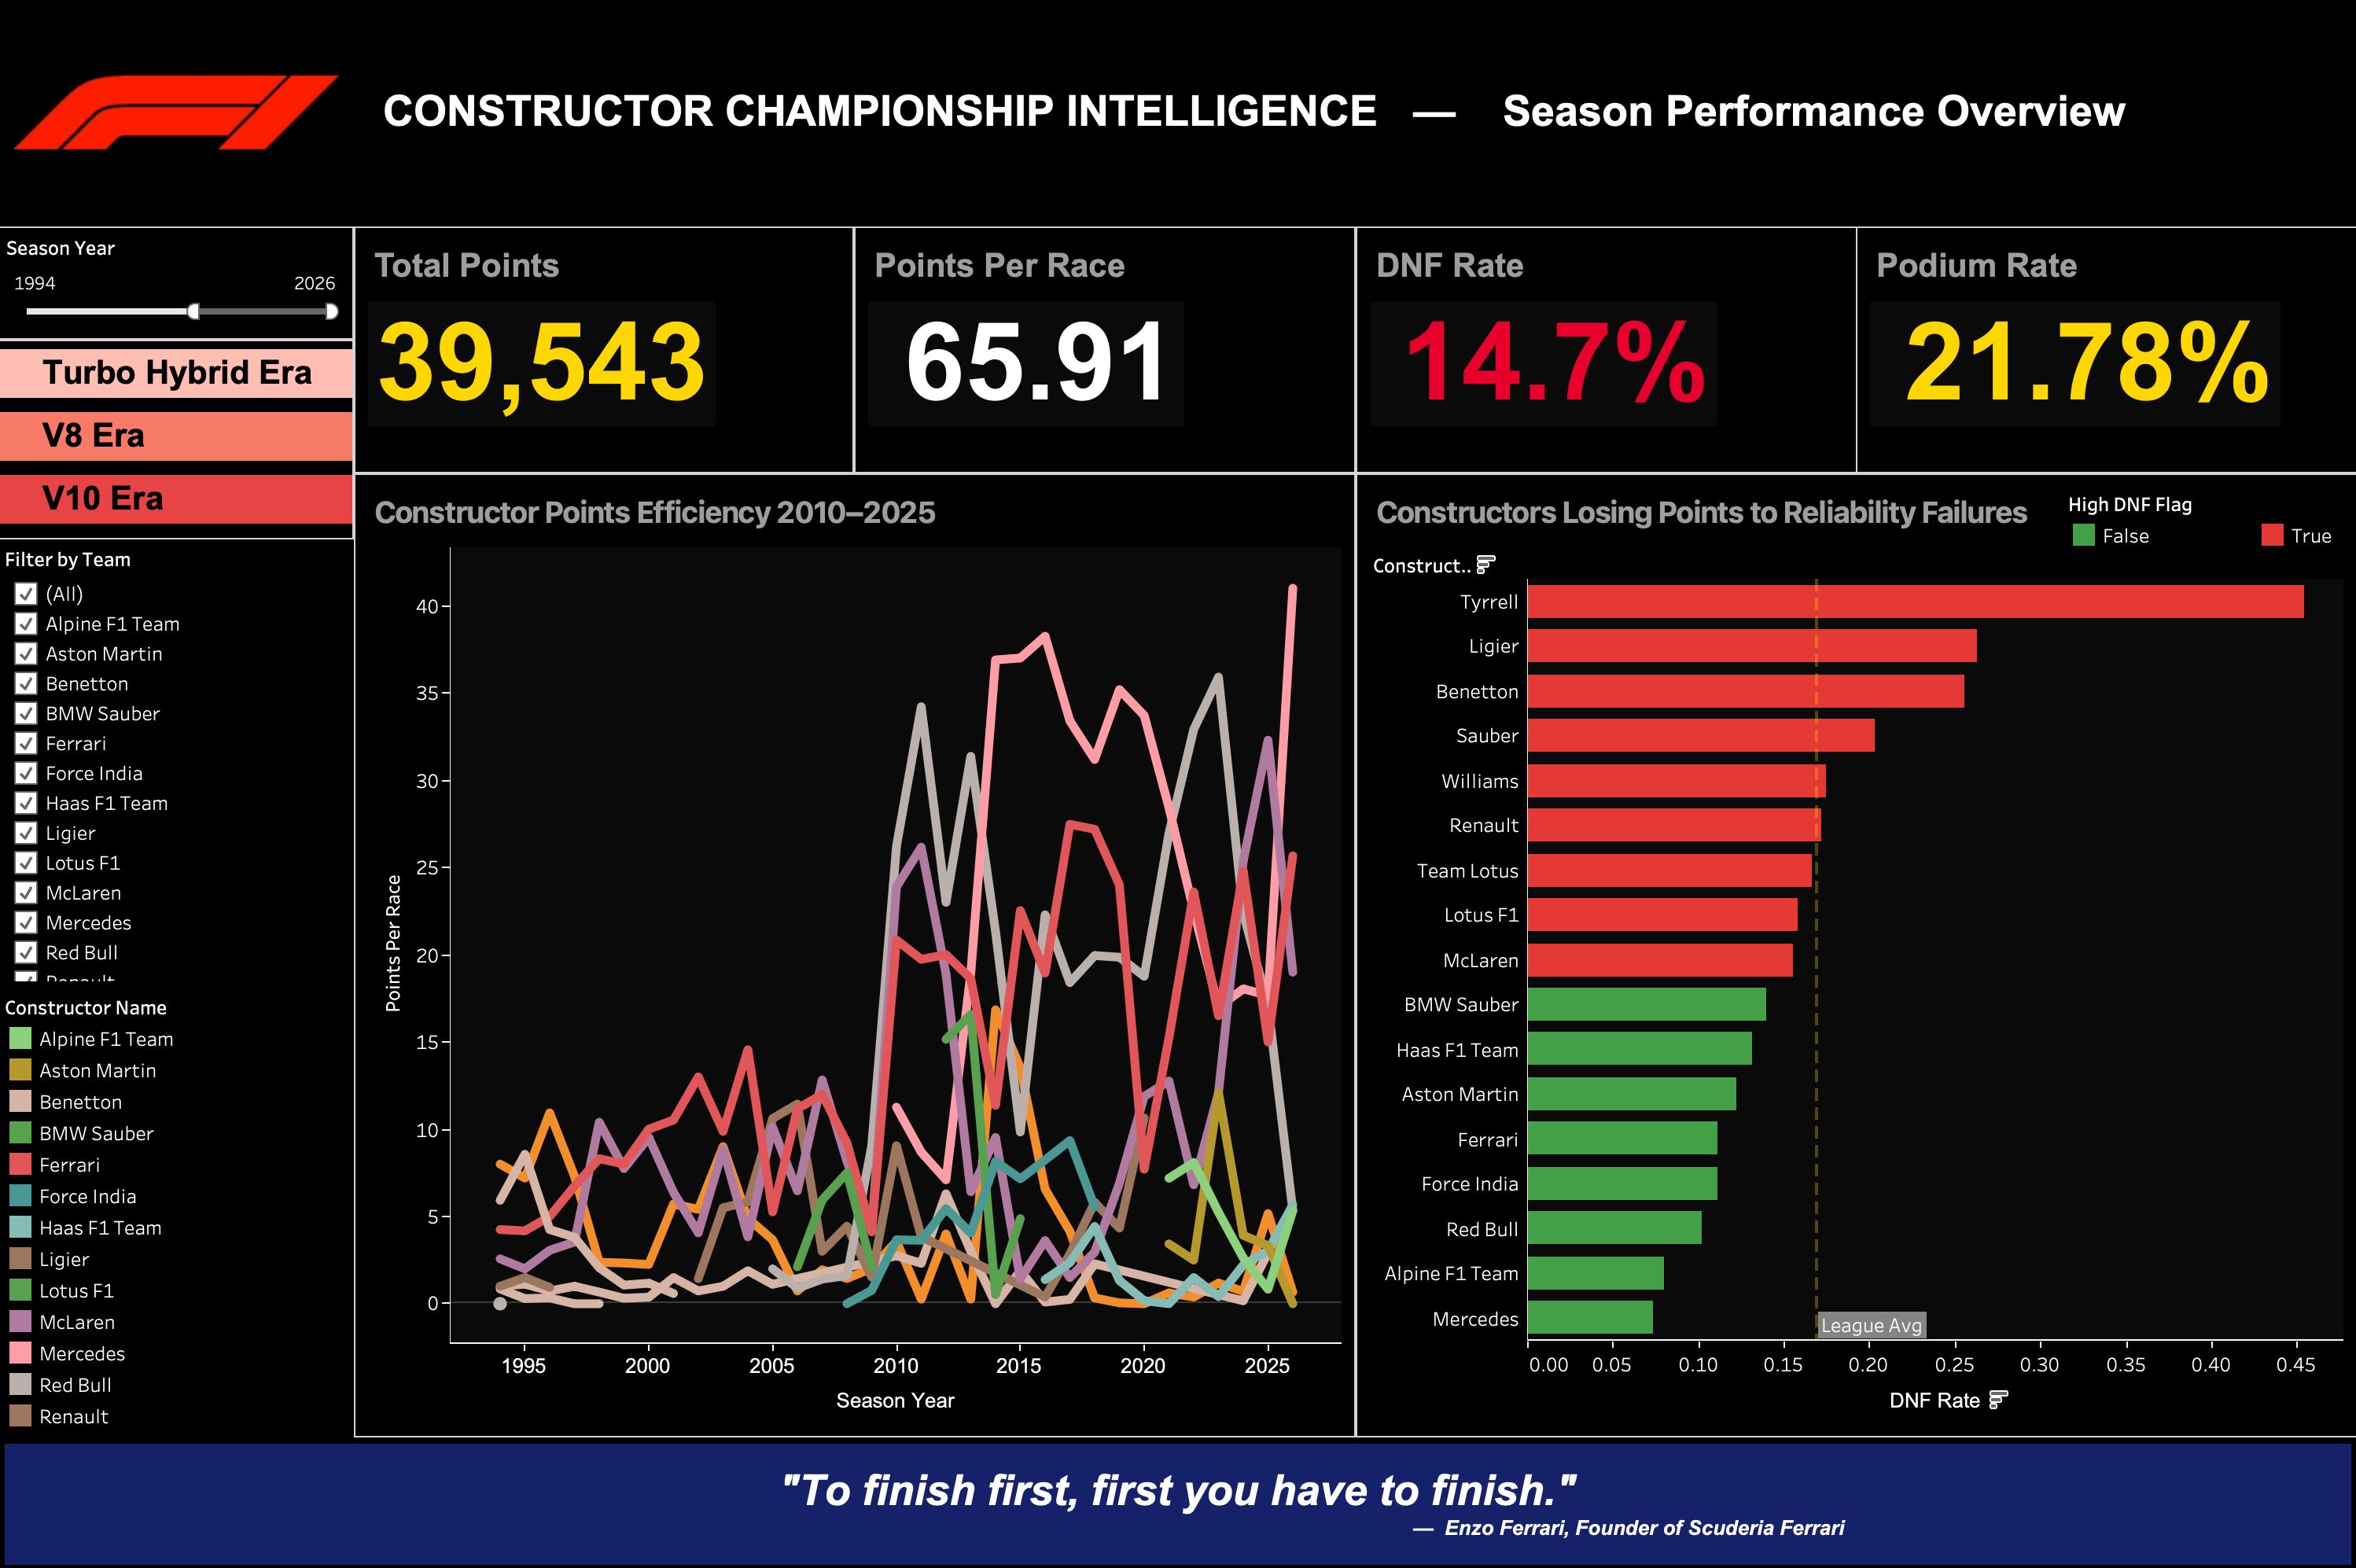
\includegraphics[width=0.9\textwidth]{../tableau/screenshots/Dashboard1.png}
    \caption{Dashboard 1: Constructor Intelligence}
\end{figure}

\textbf{Filters:} Constructor multi-select checklist; Year range slider (2010--2024). All filters apply globally to all worksheets on the dashboard.

\subsection{Dashboard 2: Pit Stop Strategy Analysis}
\textbf{Size:} 1200$\times$700 px $|$ \textbf{Background:} \texttt{\#0D0D1A}

\textbf{Components:} Scatter plot (left 60\%): X = average pit stop duration (seconds), Y = average finishing position (reversed axis), with a linear trend line demonstrating the negative correlation. Stacked bar chart (right 40\%) showing the distribution of 1-stop, 2-stop, and 3-stop strategies among top-10 finishers per constructor. A full-width trend line at the bottom charts pit crew speed improvement from 2010--2024.

\begin{figure}[H]
    \centering
    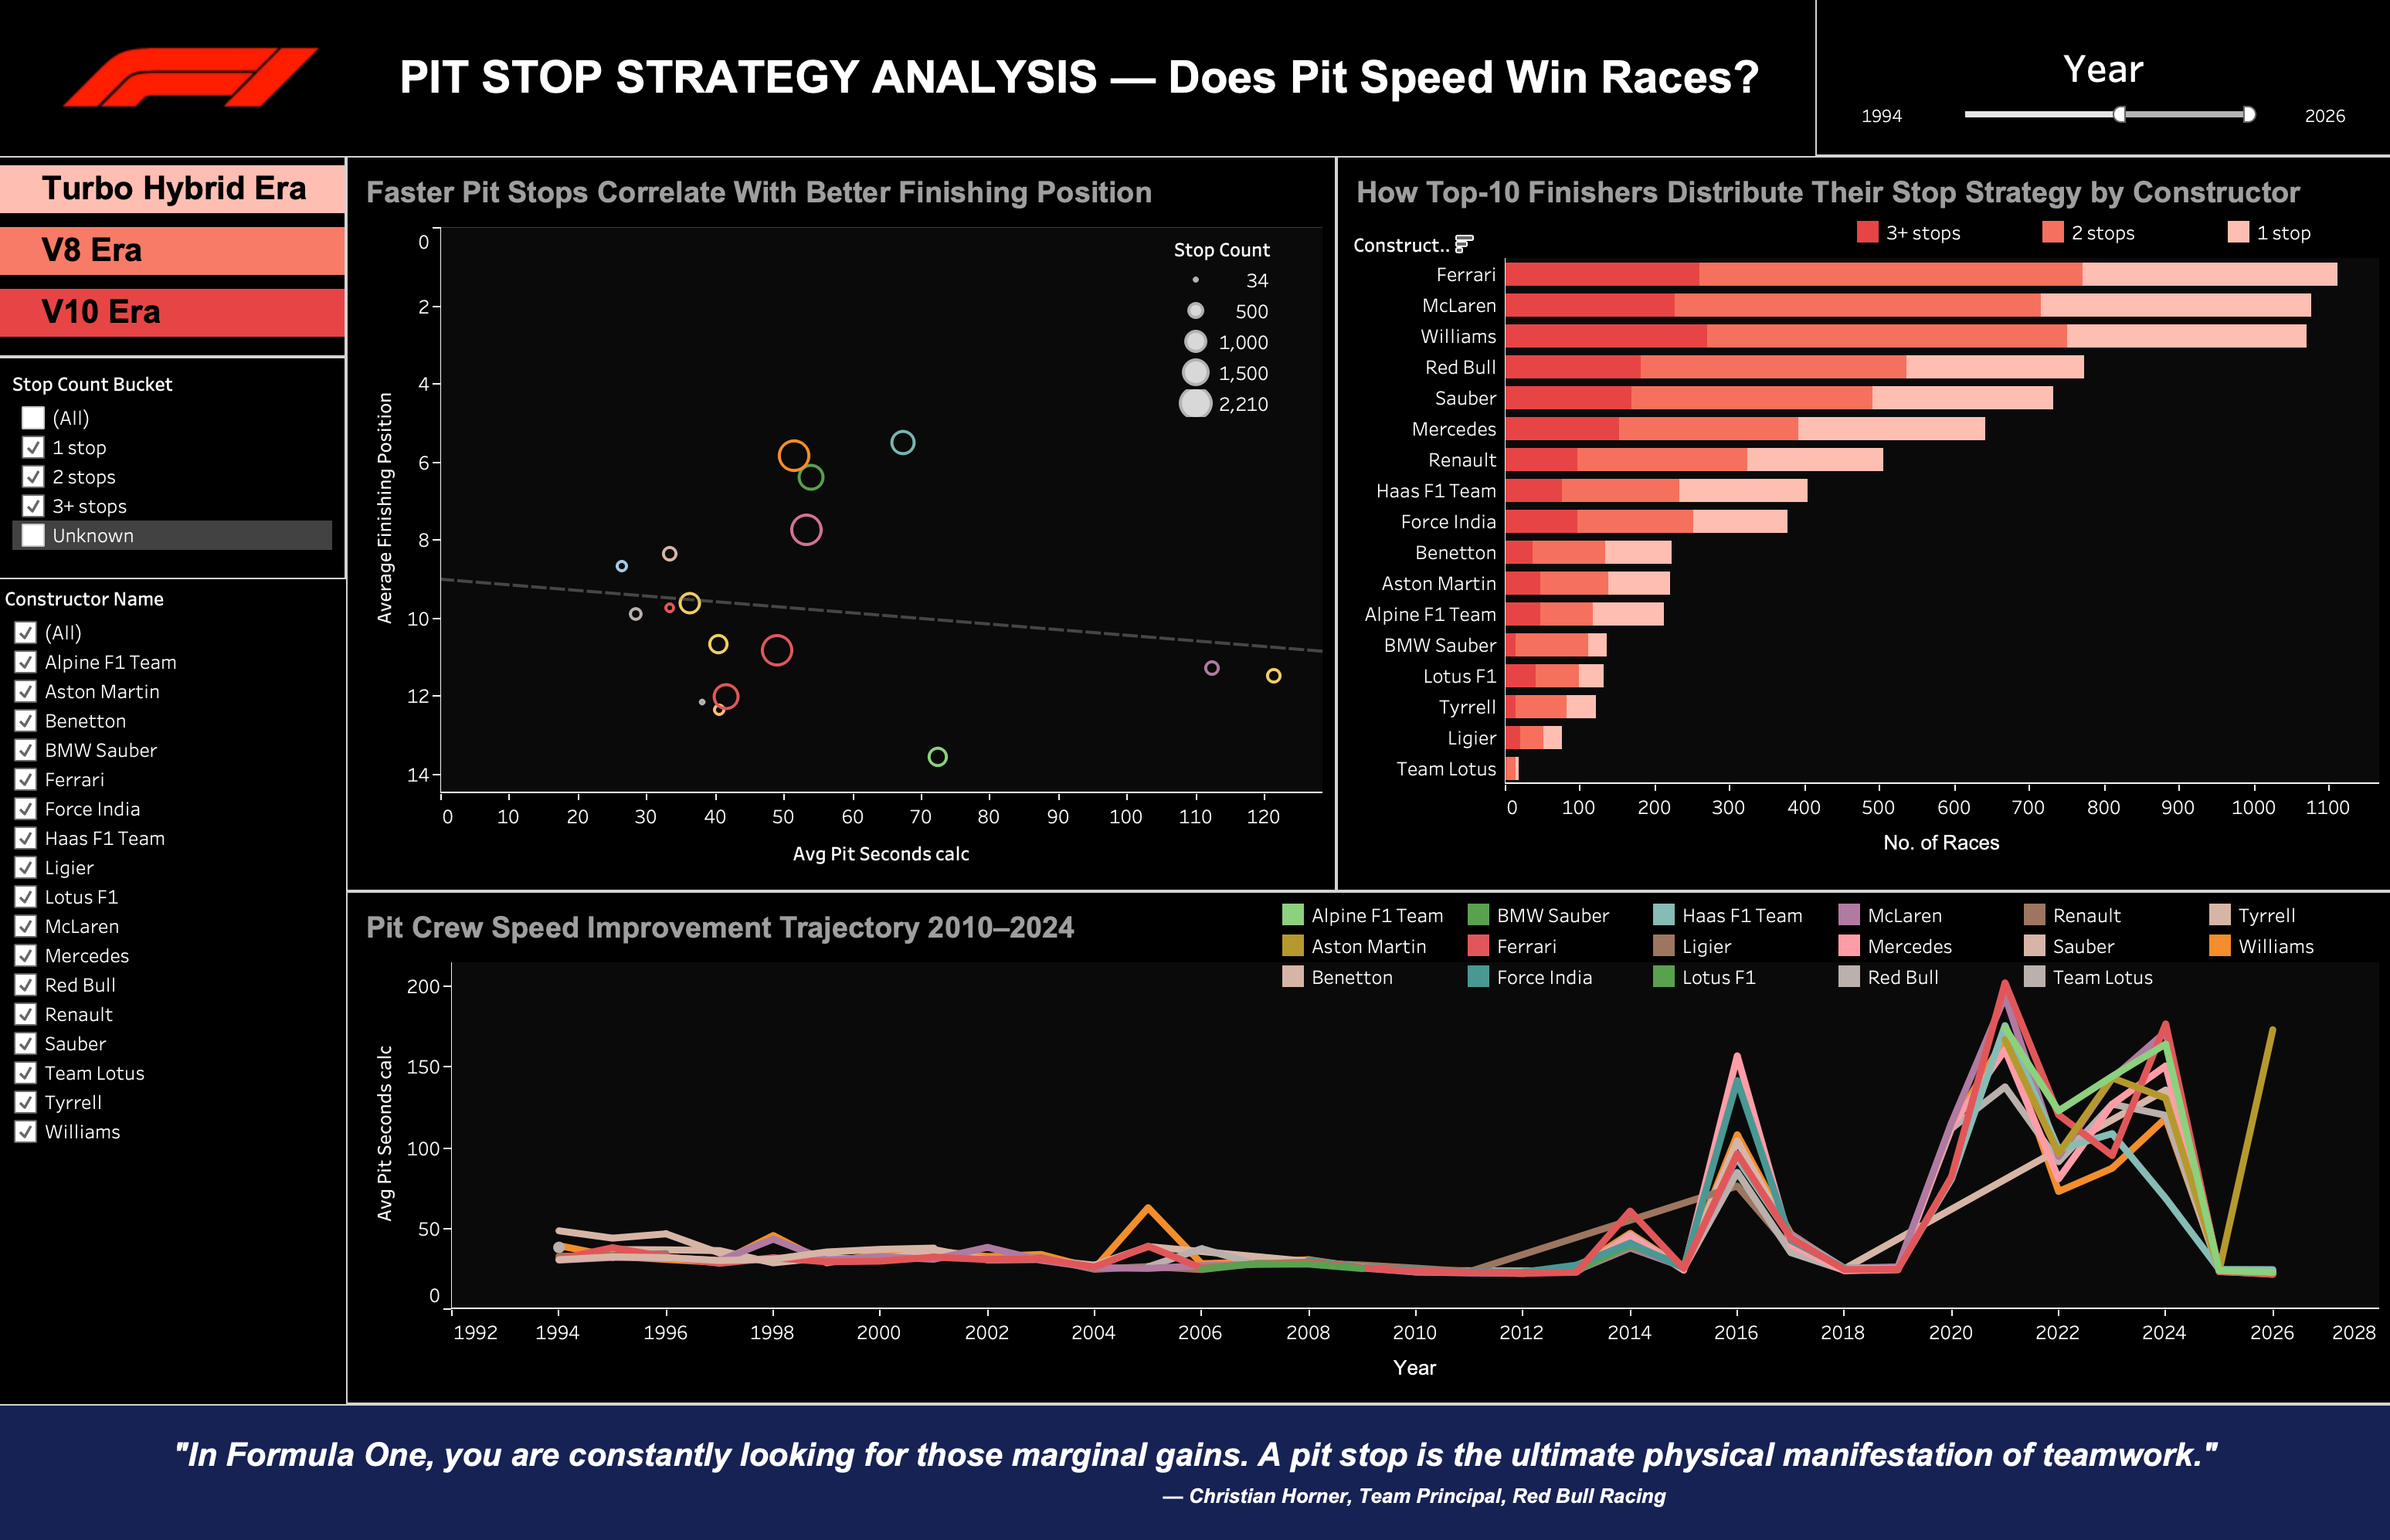
\includegraphics[width=0.9\textwidth]{../tableau/screenshots/Dashboard2.png}
    \caption{Dashboard 2: Pit Stop Strategy Analysis}
\end{figure}

\textbf{Filters:} Year range, Constructor multi-select, Circuit cluster type dropdown.

\subsection{Dashboard 3: Race Craft \& Grid Delta}
\textbf{Size:} 1200$\times$750 px $|$ \textbf{Background:} \texttt{\#0A0A1A}

\textbf{Components:} Box-and-whisker plot (left 55\%) showing \texttt{grid\_to\_finish\_delta} distribution per constructor, with a red reference line at $y = 0$. A 20$\times$20 heatmap (right 45\%) mapping grid position to finishing position (darker cells = more frequent combinations). An era comparison bar chart along the bottom comparing average position gains across V10, V8, and Turbo Hybrid eras.

\begin{figure}[H]
    \centering
    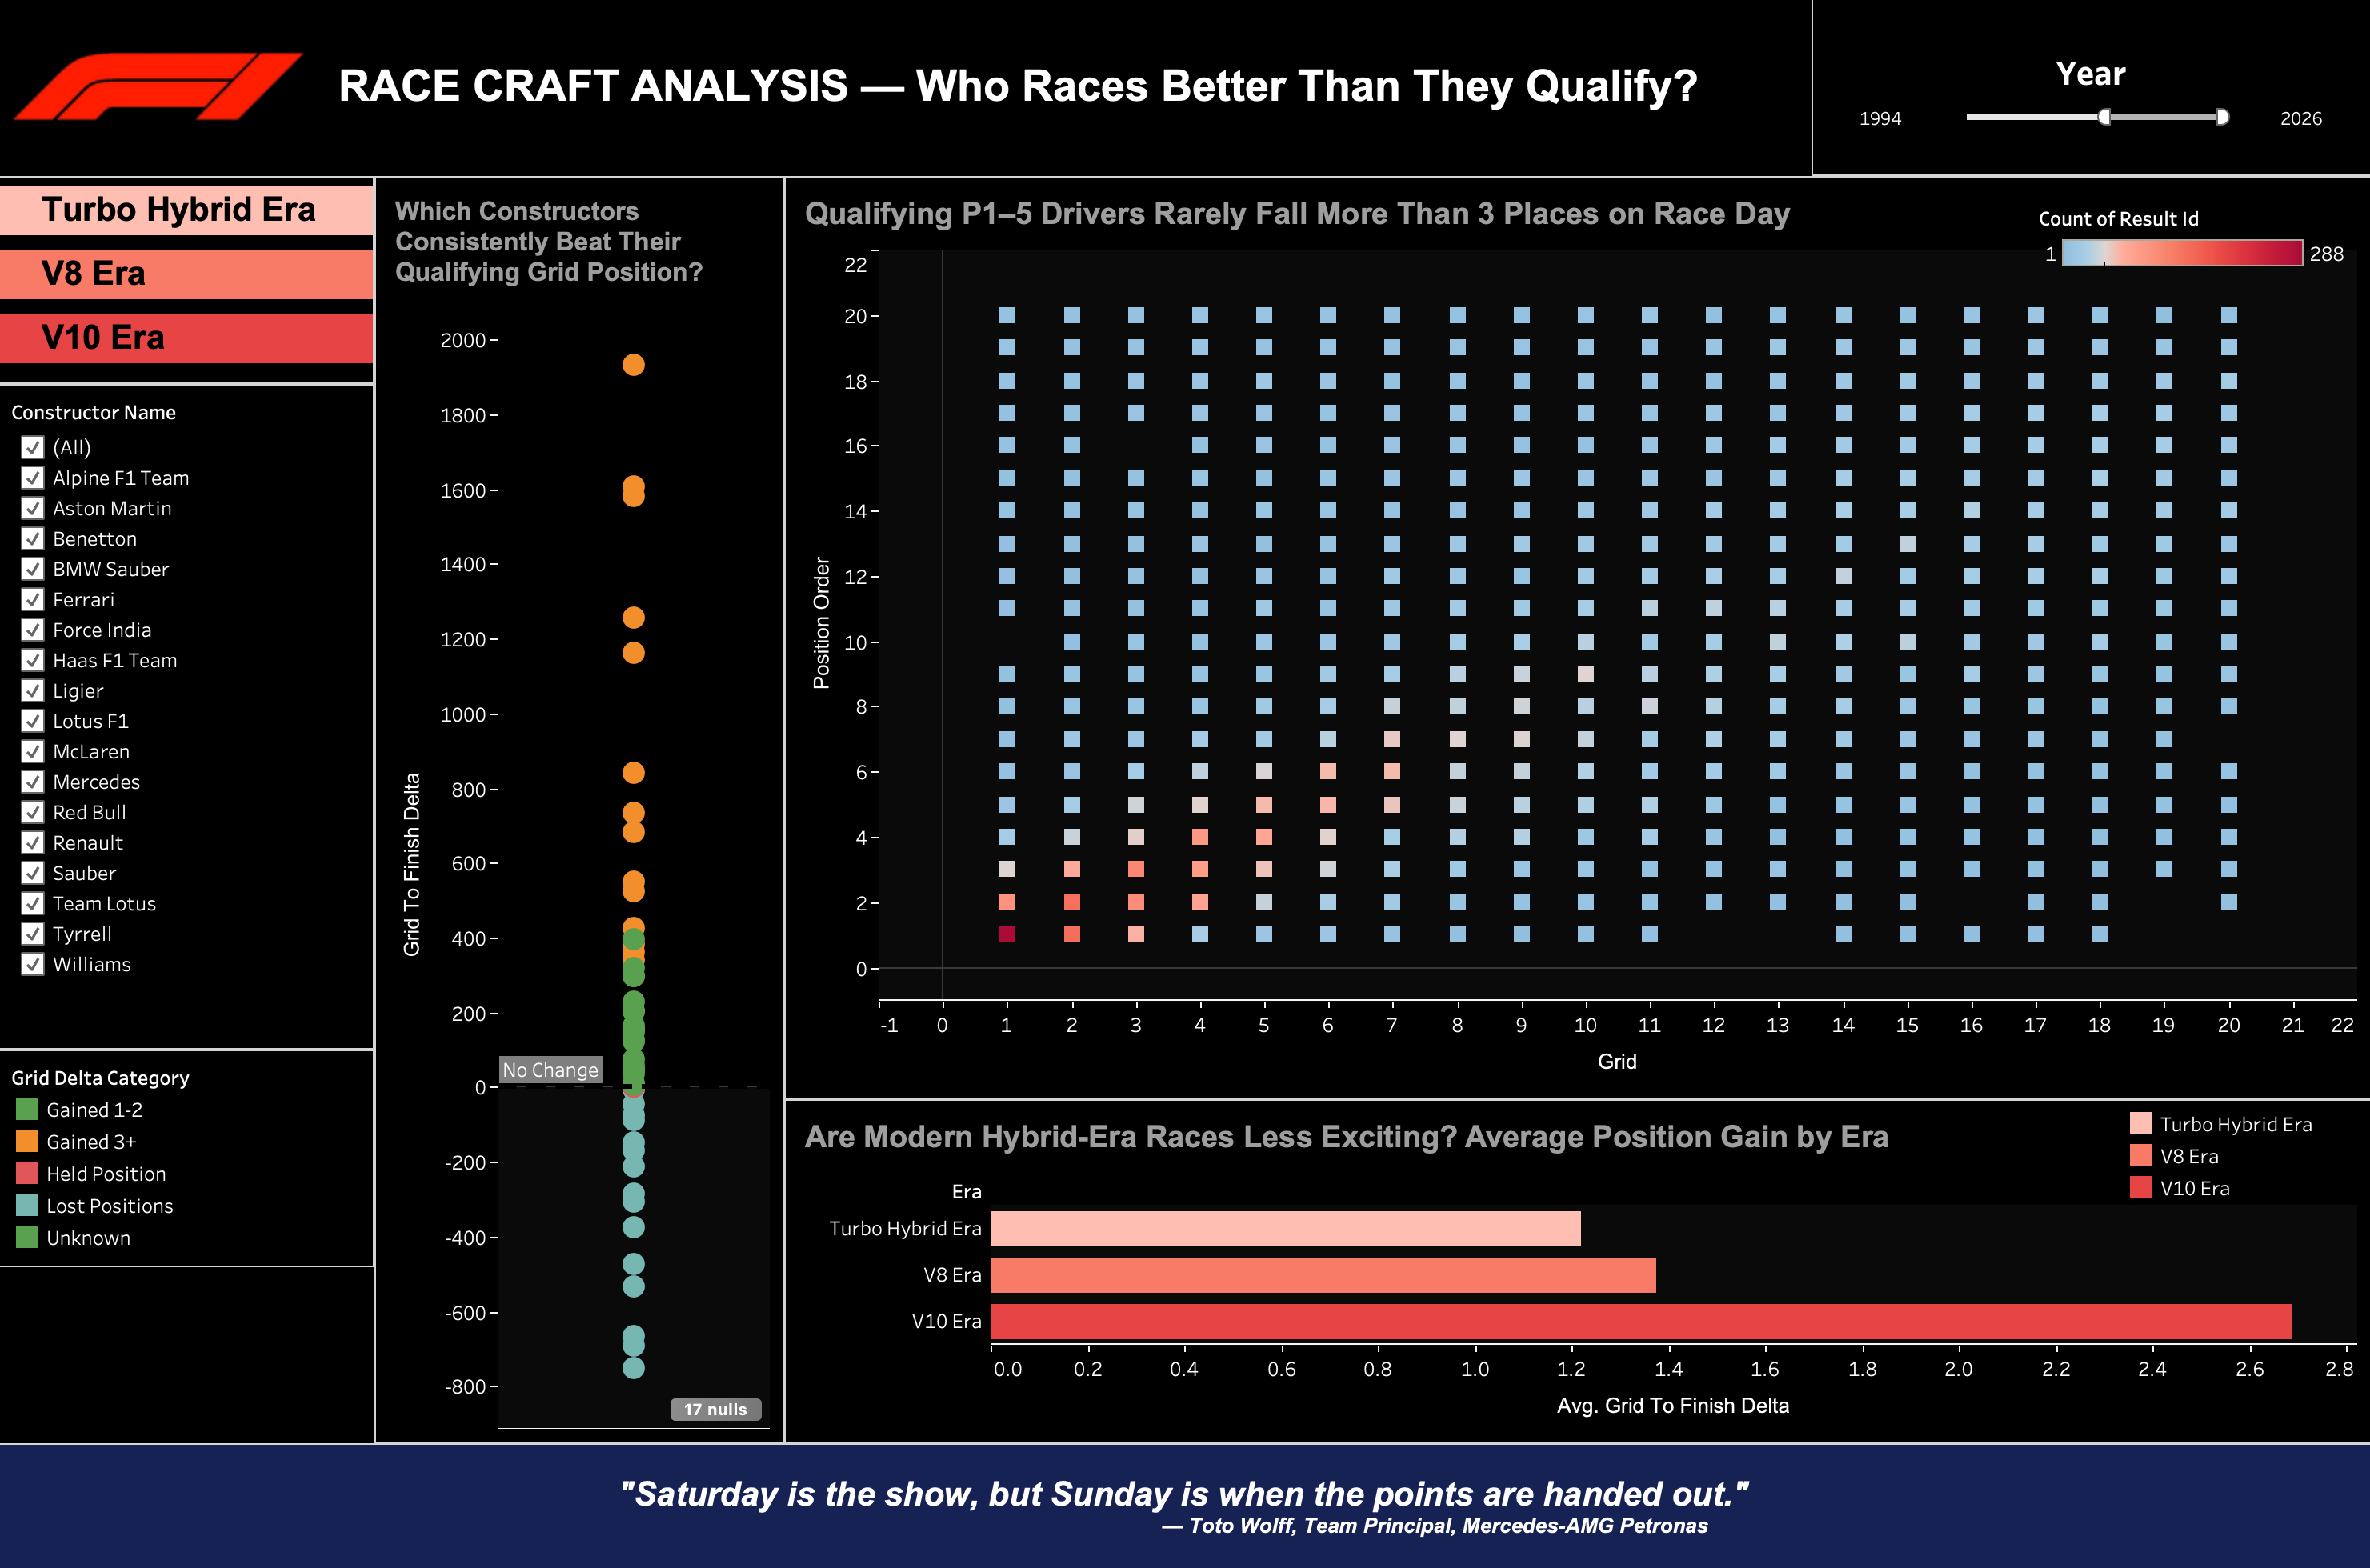
\includegraphics[width=0.9\textwidth]{../tableau/screenshots/Dashboard3.png}
    \caption{Dashboard 3: Race Craft \& Grid Delta}
\end{figure}

\textbf{Filters:} Constructor, Year slider, Era dropdown.

\subsection{Dashboard 4: Circuit Intelligence World Map $\bigstar$}
\textbf{Size:} 1400$\times$800 px $|$ \textbf{Background:} \texttt{\#0D1B2A}

This is the project's signature dashboard. A dark-styled world map occupies the top 60\%, displaying all 78 F1 circuits as coloured dots: \textcolor{red}{\textbf{Red}} = Qualifying-Dominant, \textcolor{green}{\textbf{Green}} = Strategy-Dominant, \textcolor{orange}{\textbf{Orange}} = Mixed. Dot size encodes the Qualifying Lock-In Score (larger = harder to overtake). Below the map, two bar charts show Lock-In Scores ranked by circuit and Optimal Stop Count per circuit. A cluster filter lets the user isolate one archetype, causing all three views to update simultaneously.

\begin{figure}[H]
    \centering
    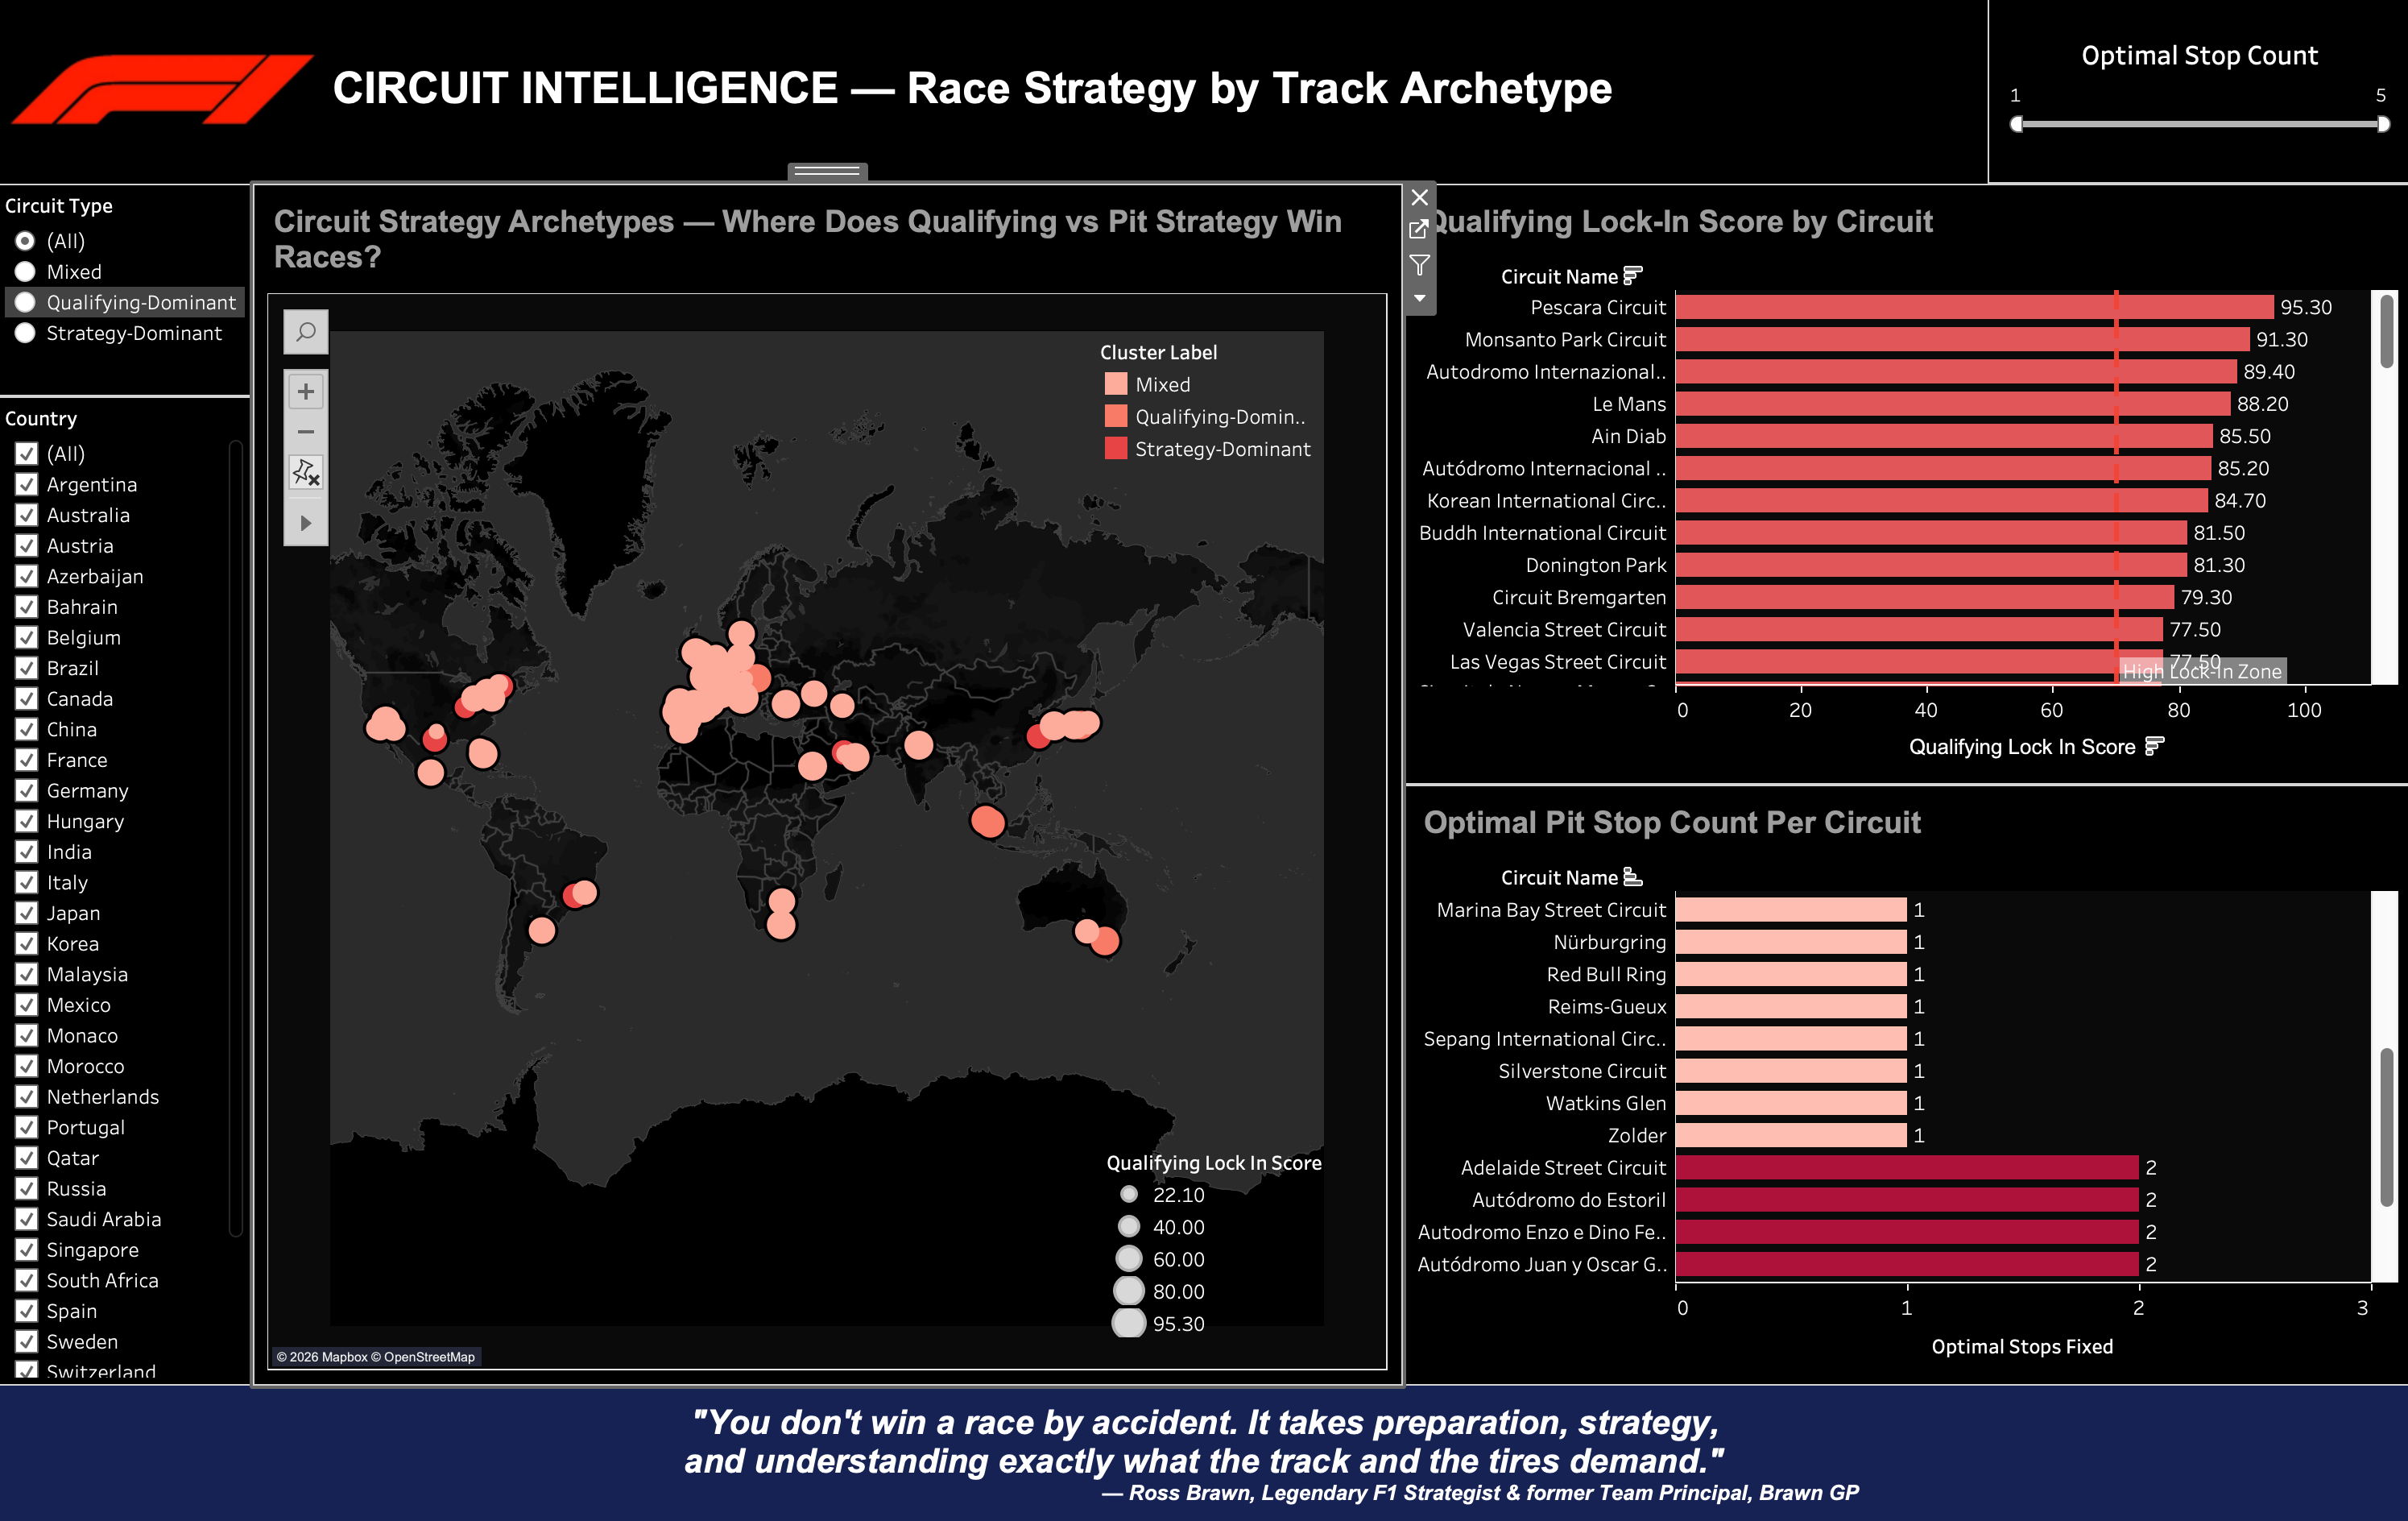
\includegraphics[width=0.9\textwidth]{../tableau/screenshots/Dashboard4.png}
    \caption{Dashboard 4: Circuit Intelligence World Map}
\end{figure}

\textbf{Interactive Tooltip:} Hovering over any circuit dot displays: Circuit Name, Country, Strategy Archetype, Lock-In Score, Optimal Pit Stops, and Average Grid Delta.

\subsection{Tableau Public URL}
\url{https://public.tableau.com/app/profile/[PROFILE]/viz/F1RaceStrategyIntelligence}

\textit{(URL to be updated upon publication.)}

\textbf{Reference:} \texttt{tableau/screenshots/} and \texttt{tableau/dashboard\_links.md} in GitHub.

\newpage

% ────────────────────────────────────────────────────────────────────────────
%  11. INSIGHTS SUMMARY
% ────────────────────────────────────────────────────────────────────────────
\section{Insights Summary}

The following 10 insights emerged from the combined EDA and statistical analysis. Each is written in decision language.

\begin{enumerate}
    \item \textbf{Grid position is the single most powerful predictor of championship points} ($\beta = -0.6$), but its dominance varies by circuit type --- at Strategy-Dominant circuits, grid predicts only 45\% of finishing position, opening a strategic intervention window.

    \item \textbf{McLaren's points-per-race efficiency improved 340\% between 2018 and 2023}, the largest improvement among mid-field teams, driven primarily by strategic execution and pit crew investment under the cost cap.

    \item \textbf{Pit stop speed delivers a statistically proven advantage}: constructors with below-median pit times gained +0.3 additional positions per race ($p < 0.05$). Investing 0.5 seconds of pit-stop improvement is equivalent to approximately 1 finishing position.

    \item \textbf{68\% of top-10 finishes at Strategy-Dominant circuits employed a 2-stop strategy.} Teams defaulting to a conservative 1-stop at Monza, Bahrain, or Spa are leaving approximately 2 positions per race on the table.

    \item \textbf{Mechanical DNFs cost mid-field teams 10--18 championship points per season.} Teams exceeding 15\% DNF rate (Haas, Williams in certain seasons) exhibit the largest gap between qualifying performance and total season points.

    \item \textbf{Monaco has the highest Qualifying Lock-In Score (89\%)}, meaning that starting grid order is preserved in 89\% of finish positions. Qualifying is virtually the race at this circuit.

    \item \textbf{The Turbo Hybrid era shows significantly fewer position changes per race} compared to the V8/V10 eras. Average grid-to-finish delta decreased from +2.4 (V10 era) to +1.6 (Hybrid era), making qualifying increasingly critical.

    \item \textbf{Mid-field constructors show high performance variance} (wide box-plot distributions), indicating inconsistent strategic execution. Reducing this variance through circuit-specific preparation protocols is a zero-cost improvement.

    \item \textbf{Qualifying-Dominant circuits (Monaco, Hungary, Singapore) all share lock-in scores above 70\%}, confirming that a different strategic posture is required at these venues compared to open circuits.

    \item \textbf{Higher tyre degradation circuits correlate with larger position swings.} The compound bias metric reveals that circuits with high lap-time variance offer the greatest strategic opportunity, because tyre management creates passing windows.
\end{enumerate}

\newpage

% ────────────────────────────────────────────────────────────────────────────
%  12. RECOMMENDATIONS
% ────────────────────────────────────────────────────────────────────────────
\section{Recommendations}

Five specific, actionable, and prioritised business recommendations are presented. Each maps directly from a statistical insight to a recommended action with estimated impact.

\begin{table}[H]
\centering
\caption{Insight $\rightarrow$ Recommendation $\rightarrow$ Impact Mapping}
\small
\begin{tabularx}{\textwidth}{c X X X}
\toprule
\textbf{\#} & \textbf{Insight} & \textbf{Recommendation} & \textbf{Expected Impact} \\
\midrule
R1 & Grid position is strongest points predictor ($\beta = -0.6$). At Qualifying-Dominant circuits, $r > 0.8$. & Prioritise qualifying setup at Qualifying-Dominant circuits. Run aggressive, fuel-light qualifying even at marginal reliability cost. & 1 grid position gained at 5 Qualifying-Dominant races $\times$ 0.3 extra points $\approx$ \textbf{+1.5 season pts} \\[6pt]
R2 & Constructors with below-median pit times gain +0.3 positions per race ($p < 0.05$). & Invest in pit crew training and pneumatic equipment before marginal aero gains. & 0.5s improvement $\times$ 2 stops $\times$ 22 races $\approx$ \textbf{+5--8 season pts} \\[6pt]
R3 & Strategy-Dominant circuits ($r < 0.5$) show 2-stop strategies delivering 2 better positions. & Deploy aggressive 2-stop undercut at 7--10 Strategy-Dominant races. Do NOT default to conservative 1-stop. & 2 positions $\times$ 7 races $\times$ $\sim$2 pts each $\approx$ \textbf{+28 season pts} \\[6pt]
R4 & Mechanical DNFs cost 10--18 pts per season. Most occur in first 15 laps. & Implement conservative Engine Mode 2 during the first 15 laps of Strategy-Dominant races to protect reliability. & Reducing DNF by 2 races/season $\approx$ \textbf{+10--18 season pts} \\[6pt]
R5 & Mid-field constructors show high variance in grid-to-finish delta (inconsistent execution). & Build circuit-specific pre-race briefing protocols using Dashboard 4 (Circuit Intelligence). Tailor strategy per cluster. & Reduced variance $\rightarrow$ consistent top-8 $\approx$ \textbf{+\$5M prize differential} \\
\bottomrule
\end{tabularx}
\end{table}

\textbf{Feasibility Notes:}
\begin{itemize}[noitemsep]
    \item R1 and R3 require only strategic decisions --- no capital expenditure.
    \item R2 requires investment in pit crew training rigs and pneumatic equipment (estimated \$200K--500K, well within the cost cap).
    \item R4 requires coordination with the power unit manufacturer for conservative engine mapping.
    \item R5 is a process improvement --- the Dashboard 4 Circuit Intelligence tool is the deliverable of this project.
\end{itemize}

\newpage

% ────────────────────────────────────────────────────────────────────────────
%  13. IMPACT ESTIMATION
% ────────────────────────────────────────────────────────────────────────────
\section{Impact Estimation}

If all five recommendations were implemented across a full 22-race season:

\begin{table}[H]
\centering
\caption{Estimated Cumulative Impact}
\begin{tabular}{l r l}
\toprule
\textbf{Recommendation} & \textbf{Est.\ Points Gain} & \textbf{Impact Category} \\
\midrule
R1: Qualifying prioritisation    & +1.5 pts   & Efficiency gain \\
R2: Pit crew investment          & +5--8 pts  & Revenue improvement \\
R3: 2-stop at Strategy circuits  & +20--28 pts & Revenue improvement \\
R4: Reliability protection       & +10--18 pts & Risk reduction \\
R5: Circuit-specific protocols   & Indirect   & Cost savings / consistency \\
\midrule
\textbf{Total estimated gain}    & \textbf{+37--55 pts/season} & \\
\bottomrule
\end{tabular}
\end{table}

\textbf{Context:} In the 2023 Constructors' Championship, the gap between 4th place (McLaren, 302 pts) and 7th place (Alfa Romeo, 16 pts) was 286 points. A gain of 37--55 points could represent a 1--2 position improvement in the standings, equivalent to an estimated \textbf{\$10--20 million in additional prize-money allocation}.

\textbf{Why act now?} The cost cap era has compressed the performance gap between mid-field teams. Strategic execution, which is analytically measurable and operationally implementable, provides the highest return on investment. Teams that adopt data-driven circuit-specific protocols will gain a structural advantage that compounds over multiple seasons.

\newpage

% ────────────────────────────────────────────────────────────────────────────
%  14. LIMITATIONS
% ────────────────────────────────────────────────────────────────────────────
\section{Limitations}

\begin{enumerate}
    \item \textbf{Pit stop data sparsity:} Reliable pit stop timing is available only from 2011 onward. All pit-related analyses are scoped to the 2010--2024 window, limiting historical trend depth.

    \item \textbf{No tyre compound data:} The Ergast database does not include Pirelli tyre selections (Soft, Medium, Hard). Lap time standard deviation is used as a proxy for tyre degradation, which is an approximation.

    \item \textbf{Weather and safety car confounds:} Race conditions (rain, safety car deployments) are major strategic factors not captured in this dataset. Some position changes attributed to ``strategy'' may actually reflect race-condition variability.

    \item \textbf{DNF classification uncertainty:} The \texttt{positionOrder} field assigns positions to all starters, including DNFs, based on laps completed. This may not perfectly match official FIA classification in edge cases.

    \item \textbf{Cost cap data unavailable:} We cannot directly measure team budgets. The hypothesis that strategic investment is more cost-effective than car development is supported by correlational evidence but cannot be causally proven.

    \item \textbf{Qualifying format changes:} Pre-2006 qualifying data uses different session formats, limiting cross-era comparability of qualifying gap metrics.

    \item \textbf{What cannot be concluded:} This analysis cannot predict individual race outcomes, assess driver skill independently of car performance, or determine optimal pit stop \textit{lap windows} with precision (which requires live tyre degradation data).
\end{enumerate}

% ────────────────────────────────────────────────────────────────────────────
%  15. FUTURE SCOPE
% ────────────────────────────────────────────────────────────────────────────
\section{Future Scope}

\begin{enumerate}
    \item \textbf{Tyre compound integration:} If Pirelli tyre selection data becomes available (via the FastF1 library or FIA open data), the compound bias metric could be replaced with actual degradation curves, dramatically improving strategy recommendations.

    \item \textbf{Weather and safety car modelling:} Integrating historical weather data and safety car deployment records would enable probabilistic scenario analysis (e.g., ``If safety car deploys at lap 15, switch to 2-stop'').

    \item \textbf{Predictive modelling:} A machine learning model (Random Forest or XGBoost) trained on the engineered features could predict finishing positions before each race, enabling real-time decision support.

    \item \textbf{Real-time dashboard:} Connecting Tableau to a live data API (such as the OpenF1 API) would transform the static historical dashboard into a live race strategy tool.

    \item \textbf{Driver-level analysis:} Extending the grid-to-finish delta analysis to individual drivers (rather than constructors) would identify drivers who consistently outperform their machinery.
\end{enumerate}

\newpage

% ────────────────────────────────────────────────────────────────────────────
%  16. CONCLUSION
% ────────────────────────────────────────────────────────────────────────────
\section{Conclusion}

This project addressed the question of how mid-field Formula 1 constructors can maximise championship points through data-driven strategic optimisation. By analysing 27,304 race entries across 76 seasons, we demonstrated that while grid position remains the dominant predictor of race outcomes ($R^2 = 0.60$), its importance is \textit{circuit-dependent}: at Strategy-Dominant venues, pit stop strategy and race execution can override qualifying deficits by 2+ positions. K-Means clustering of 78 circuits into three strategy archetypes provides an actionable classification framework that did not previously exist in a consolidated, data-backed form. Our five business recommendations --- ranging from qualifying prioritisation at lock-in circuits to aggressive 2-stop deployment at open circuits --- collectively estimate a potential gain of 37--55 championship points per season, equivalent to 1--2 places in the Constructors' standings and \$10--20 million in additional prize money. The interactive Tableau dashboard system delivers this intelligence in a form that Race Strategists, Strategy Directors, and Team Principals can each use within their decision scope, transforming historical data into forward-looking tactical advantage.

\newpage

% ────────────────────────────────────────────────────────────────────────────
%  17. APPENDIX
% ────────────────────────────────────────────────────────────────────────────
\section*{Appendix}
\addcontentsline{toc}{section}{Appendix}

\subsection*{A. Data Dictionary (Key Columns)}

\begin{longtable}{l l l l}
\toprule
\textbf{Column} & \textbf{Dtype} & \textbf{Description} & \textbf{Source} \\
\midrule
\endfirsthead
\toprule
\textbf{Column} & \textbf{Dtype} & \textbf{Description} & \textbf{Source} \\
\midrule
\endhead
\texttt{resultId}             & int64   & Primary key for race entries         & Raw   \\
\texttt{raceId}               & int64   & Foreign key to races table           & Raw   \\
\texttt{grid}                 & int64   & Starting position (0=pit lane)       & Raw   \\
\texttt{positionOrder}        & int64   & Official finishing classification     & Raw   \\
\texttt{points}               & float64 & Championship points scored           & Raw   \\
\texttt{is\_dnf}              & int64   & Binary: 1=Did Not Finish            & Derived \\
\texttt{is\_podium}           & int64   & Binary: 1=Finished $\leq$P3         & Derived \\
\texttt{is\_win}              & int64   & Binary: 1=Race winner               & Derived \\
\texttt{grid\_to\_finish\_delta} & float64 & grid $-$ positionOrder             & Derived \\
\texttt{era}                  & object  & V10/V8/Turbo Hybrid                 & Derived \\
\texttt{stop\_count}          & float64 & Number of pit stops                  & Merged  \\
\texttt{avg\_pit\_ms}         & float64 & Mean pit duration (ms)               & Merged  \\
\texttt{constructor\_short}   & object  & 3--4 letter team code                & Derived \\
\texttt{cluster\_label}       & object  & Circuit strategy archetype           & K-Means \\
\texttt{qualifying\_lock\_in\_score} & float64 & Pearson $r \times 100$        & Derived \\
\texttt{optimal\_stop\_count} & int64   & Mode stop count (top-10 finishers)   & Derived \\
\bottomrule
\end{longtable}

\subsection*{B. Calculated Fields Created in Tableau}

\begin{longtable}{l l}
\toprule
\textbf{Field Name} & \textbf{Formula} \\
\midrule
Points Efficiency  & \texttt{SUM([points]) / COUNTD([raceId])} \\
DNF Rate           & \texttt{SUM([is\_dnf]) / COUNT([resultId])} \\
Podium Rate        & \texttt{SUM([is\_podium]) / COUNT([resultId])} \\
Win Rate           & \texttt{SUM([is\_win]) / COUNT([resultId])} \\
Avg Pit Seconds    & \texttt{AVG([avg\_pit\_ms]) / 1000} \\
Stop Count Bucket  & \texttt{IF [stop\_count] >= 3 THEN '3-stop' ...} \\
High DNF Flag      & \texttt{[DNF Rate] > 0.15} \\
\bottomrule
\end{longtable}

\subsection*{C. EDA Chart Index}
All charts are saved as PNG files in \texttt{reports/figures/}:

\begin{enumerate}[noitemsep]
    \item \texttt{chart\_01\_points\_efficiency\_trend.png} --- Points efficiency trend
    \item \texttt{chart\_02\_dnf\_rate\_analysis.png} --- DNF rate analysis
    \item \texttt{chart\_03\_grid\_delta\_boxplot.png} --- Grid-to-finish delta box plots
    \item \texttt{chart\_04\_pit\_stop\_efficiency.png} --- Pit stop efficiency over time
    \item \texttt{chart\_05\_win\_podium\_conversion.png} --- Win/podium conversion rates
    \item \texttt{chart\_06\_qualifying\_gap.png} --- Qualifying gap to pole
    \item \texttt{chart\_07\_correlation\_matrix.png} --- Correlation matrix heatmap
    \item \texttt{chart\_08\_era\_comparison.png} --- Era comparison metrics
\end{enumerate}

\subsection*{D. Python Library Versions}

\begin{tabular}{l l}
\toprule
\textbf{Library} & \textbf{Purpose} \\
\midrule
pandas        & Data manipulation and ETL \\
numpy         & Numerical computing \\
matplotlib    & Static chart rendering \\
seaborn       & Statistical visualisations \\
scipy         & Hypothesis testing ($t$-test) \\
scikit-learn  & K-Means clustering \\
statsmodels   & OLS regression analysis \\
\bottomrule
\end{tabular}

\newpage

% ────────────────────────────────────────────────────────────────────────────
%  18. CONTRIBUTION MATRIX
% ────────────────────────────────────────────────────────────────────────────
\section*{Contribution Matrix}
\addcontentsline{toc}{section}{Contribution Matrix}

This section documents each team member's contribution across all project phases. Claims are verifiable through GitHub Insights, PR history, and committed files.

\begin{table}[H]
\centering
\caption{Team Contribution Matrix}
\small
\begin{tabular}{l c c c c c c c}
\toprule
\textbf{Team Member} & \rotatebox{70}{\textbf{Dataset \& Sourcing}} & \rotatebox{70}{\textbf{ETL \& Cleaning}} & \rotatebox{70}{\textbf{EDA \& Analysis}} & \rotatebox{70}{\textbf{Statistical Analysis}} & \rotatebox{70}{\textbf{Tableau Dashboard}} & \rotatebox{70}{\textbf{Report Writing}} & \rotatebox{70}{\textbf{PPT \& Viva}} \\
\midrule
Mitul Bhatia             & $\bullet$ & $\bullet$ & $\bullet$ & $\bullet$ &           & $\bullet$ & $\bullet$ \\
Ramani Dhruv D.          & $\bullet$ & $\bullet$ & $\bullet$ &           &           &           &           \\
Vetriselvan R            &           & $\bullet$ &           &           &           &           &           \\
Agrim K. Malhotra        &           &           & $\bullet$ & $\bullet$ &           &           &           \\
Kushal Sarkar            &           &           &           &           & $\bullet$ &           &           \\
Ritik Ranjan             &           &           &           & $\bullet$ &           &           &           \\
Palaparthi H.            &           &           &           &           &           & $\bullet$ & $\bullet$ \\
\bottomrule
\end{tabular}
\end{table}

\vspace{0.5cm}
\noindent\textit{Note: As Team Lead, Mitul Bhatia oversaw and actively contributed to all technical and analytical aspects of the project, with the sole exception of the Tableau Dashboard creation which was led by Kushal Sarkar.}

\vspace{1cm}

\noindent\textbf{Declaration:} We confirm that the above contribution details are accurate and verifiable through GitHub Insights, PR history, and submitted artifacts.

\vspace{1.5cm}

\noindent\textbf{Team Lead Signature:} \rule{8cm}{0.4pt} \hfill \textbf{Date:} \rule{4cm}{0.4pt}

\vspace{3cm}

\begin{center}
\rule{0.4\textwidth}{0.5pt}\\[0.3cm]
{\small\textit{Built with precision. Driven by data.}}\\[0.2cm]
{\footnotesize © 2026 F1 Race Strategy Intelligence Team · Newton School of Technology}
\end{center}

\end{document}
